Les moteurs utilisés pour ce projet sont des moteurs DC à balais. Ce type de moteur ne nécessite qu'une source de tension DC pour l'alimenter, au contraire de moteurs synchrones ou asynchrones, basés sur des alimentations triphasées ou N-phasées.\\

\begin{minipage}[t]{.45\textwidth}
	\centering
	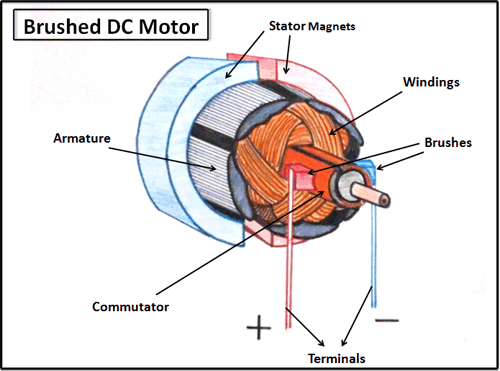
\includegraphics[width=\textwidth]{dc_motor}
	\captionof{figure}{Schéma d'un moteur DC.}
	\label{fig:dc_motor}
\end{minipage}
\hfill
\begin{minipage}[t]{.45\textwidth}
	\centering
	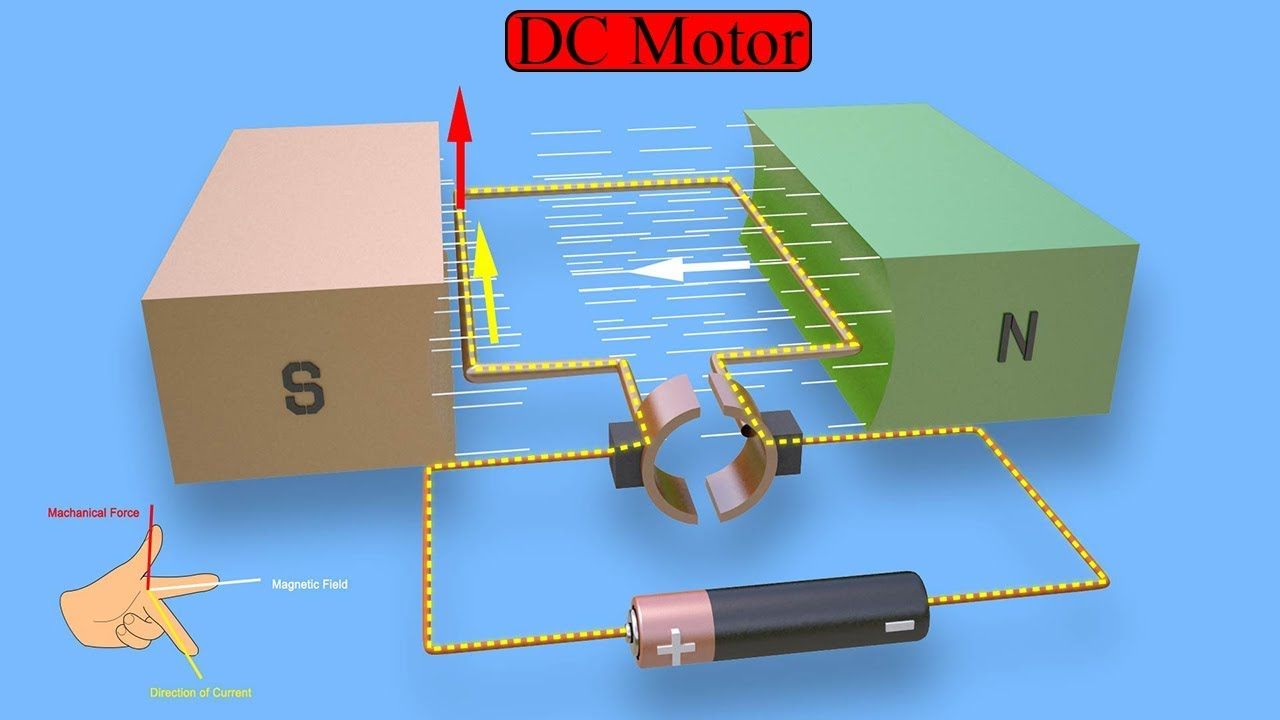
\includegraphics[width=\textwidth]{dc_motor_principle}
	\captionof{figure}{Principle de fonctionnement du moteur DC.}
	\label{fig:dc_motor_principle}
\end{minipage}
\vspace{.25cm}

Le moteur est constitué de deux pièces principales, comme illustré à la Figure \ref{fig:dc_motor}. D'une part, un \textbf{stator}, élément fixe du moteur, sur lequel on trouve généralement une structure formée d'aimants permanents, servant à générer un champ magnétique de direction fixe. D'autre part, un \textbf{rotor}, élément mobile du moteur, sur lequel on trouve généralement des bobinages alimentés par la tension DC fournie au moteur, servant à générer un champ magnétique de direction variable.\\

Le couple électro-mécanique produit par le moteur résulte du moment de force qui tend à aligner les directions des champs magnétiques générés respectivement par les aimants permanents au stator et les bobinages au rotor, comme représenté à la Figure \ref{fig:dc_motor_principle}. Un commutateur auquel les bobinages sont connectés au travers d'un système de balais, permet de choisir quels bobinages alimenter, de façon à constamment désaligner le champ magnétique résultant des bobinages par rapport à celui des aimants. C'est ce principe qui permet de produire un mouvement rotatif continu.\\

D'un point de vue purement électrique (et pour votre information uniquement, pas besoin de comprendre les détails), le fonctionnement du moteur DC est régi par 2 équations principales:

\begin{align*}
	\left \lbrace
	\begin{aligned}
		V_a &= R_a I_a + L_a \frac{dI_a}{dt} + k \phi \omega_m\\
		C_{em} &= I \frac{d\omega_m}{dt} = k \phi I_a
	\end{aligned}
	\right. 
\end{align*}

La \textbf{première équation} relie la tension d'alimentation du moteur, notée $V_a$, au courant circulant dans les bobinages, noté $I_a$ et à la force électromotric induite (le terme $k \phi \omega_m$) qui fait directement intervenir la vitesse de rotation du moteur $\omega_m$. La \textbf{seconde équation} relie le couple électro-mécanique, noté $C_{em}$ et proportionel à la dérivée de la vitesse de rotation $\frac{d\omega_m}{dt}$, au courant dans les bobinages.\\

La conclusion principale à tirer de ces équations est qu'il est possible de contrôler la vitesse du moteur $\omega_m$ uniquement en modulant la tension $V_a$ appliquée au moteur.